%!TEX root = matmul_wse.tex

\subsection{Implementation}


\begin{figure}[t!]
  \centering
  \begin{subfigure}{0.40\columnwidth}
    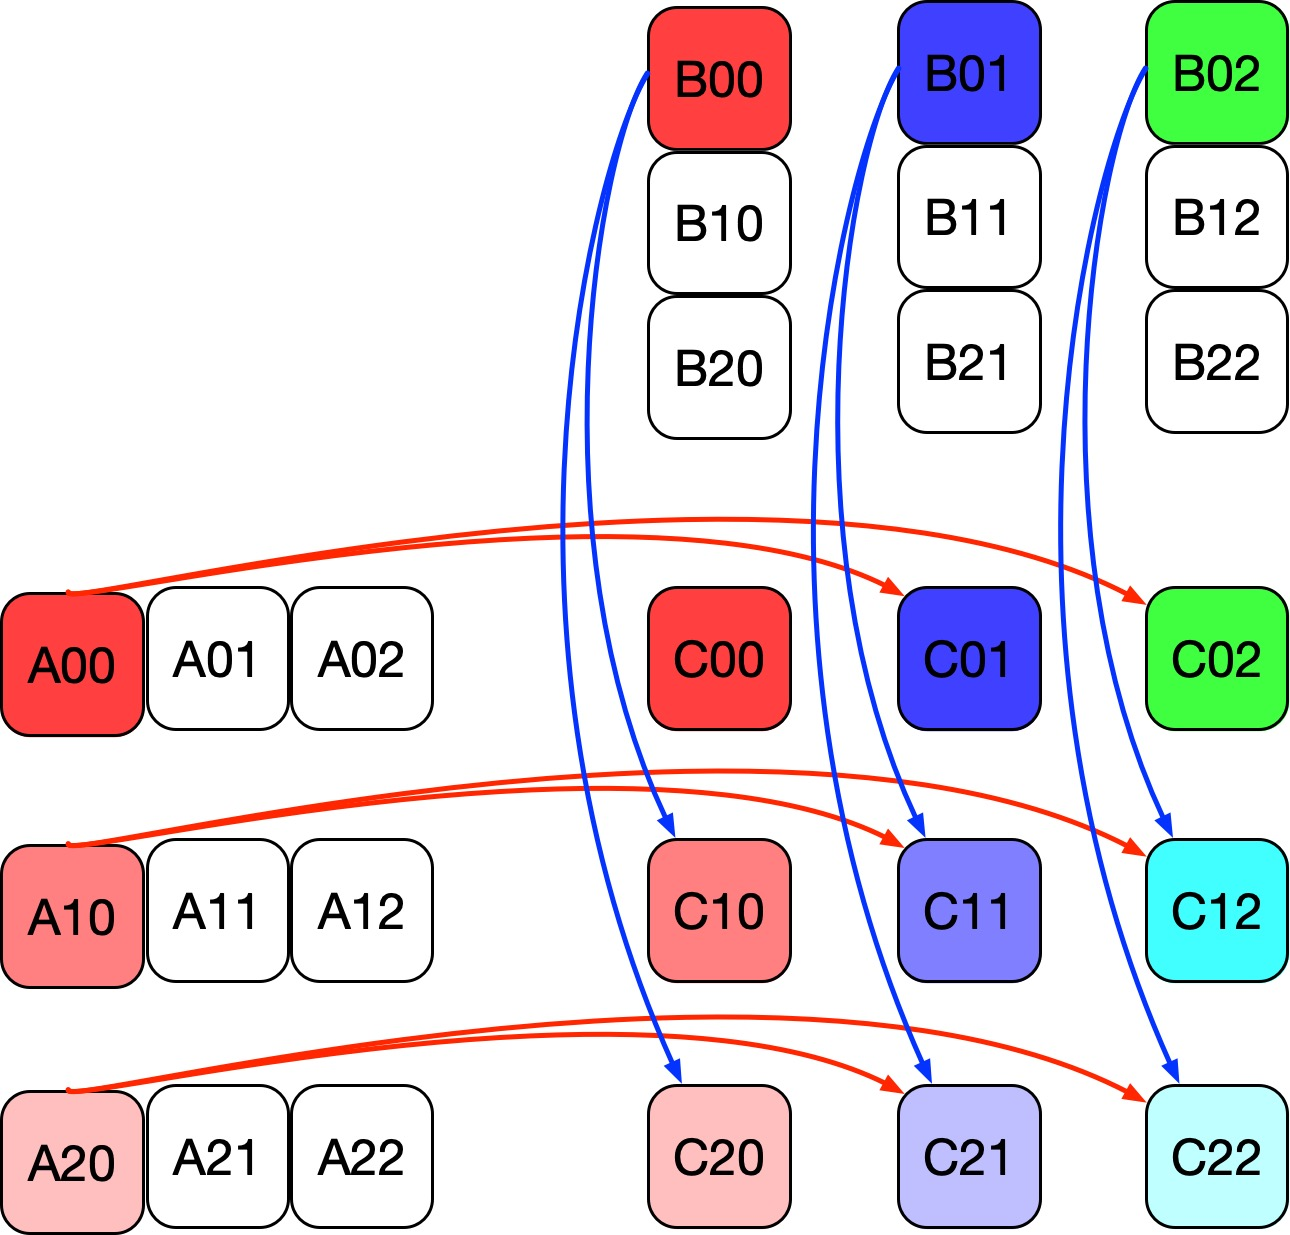
\includegraphics[width=\linewidth]{figures/gemm_summa_k0.jpg}
  \end{subfigure}
  \caption{Communication of \summa of the first iteration.}
  \label{fig:gemm_summa_k0}
\end{figure}



\begin{figure}[b!]
  \centering
  \begin{subfigure}{0.40\columnwidth}
    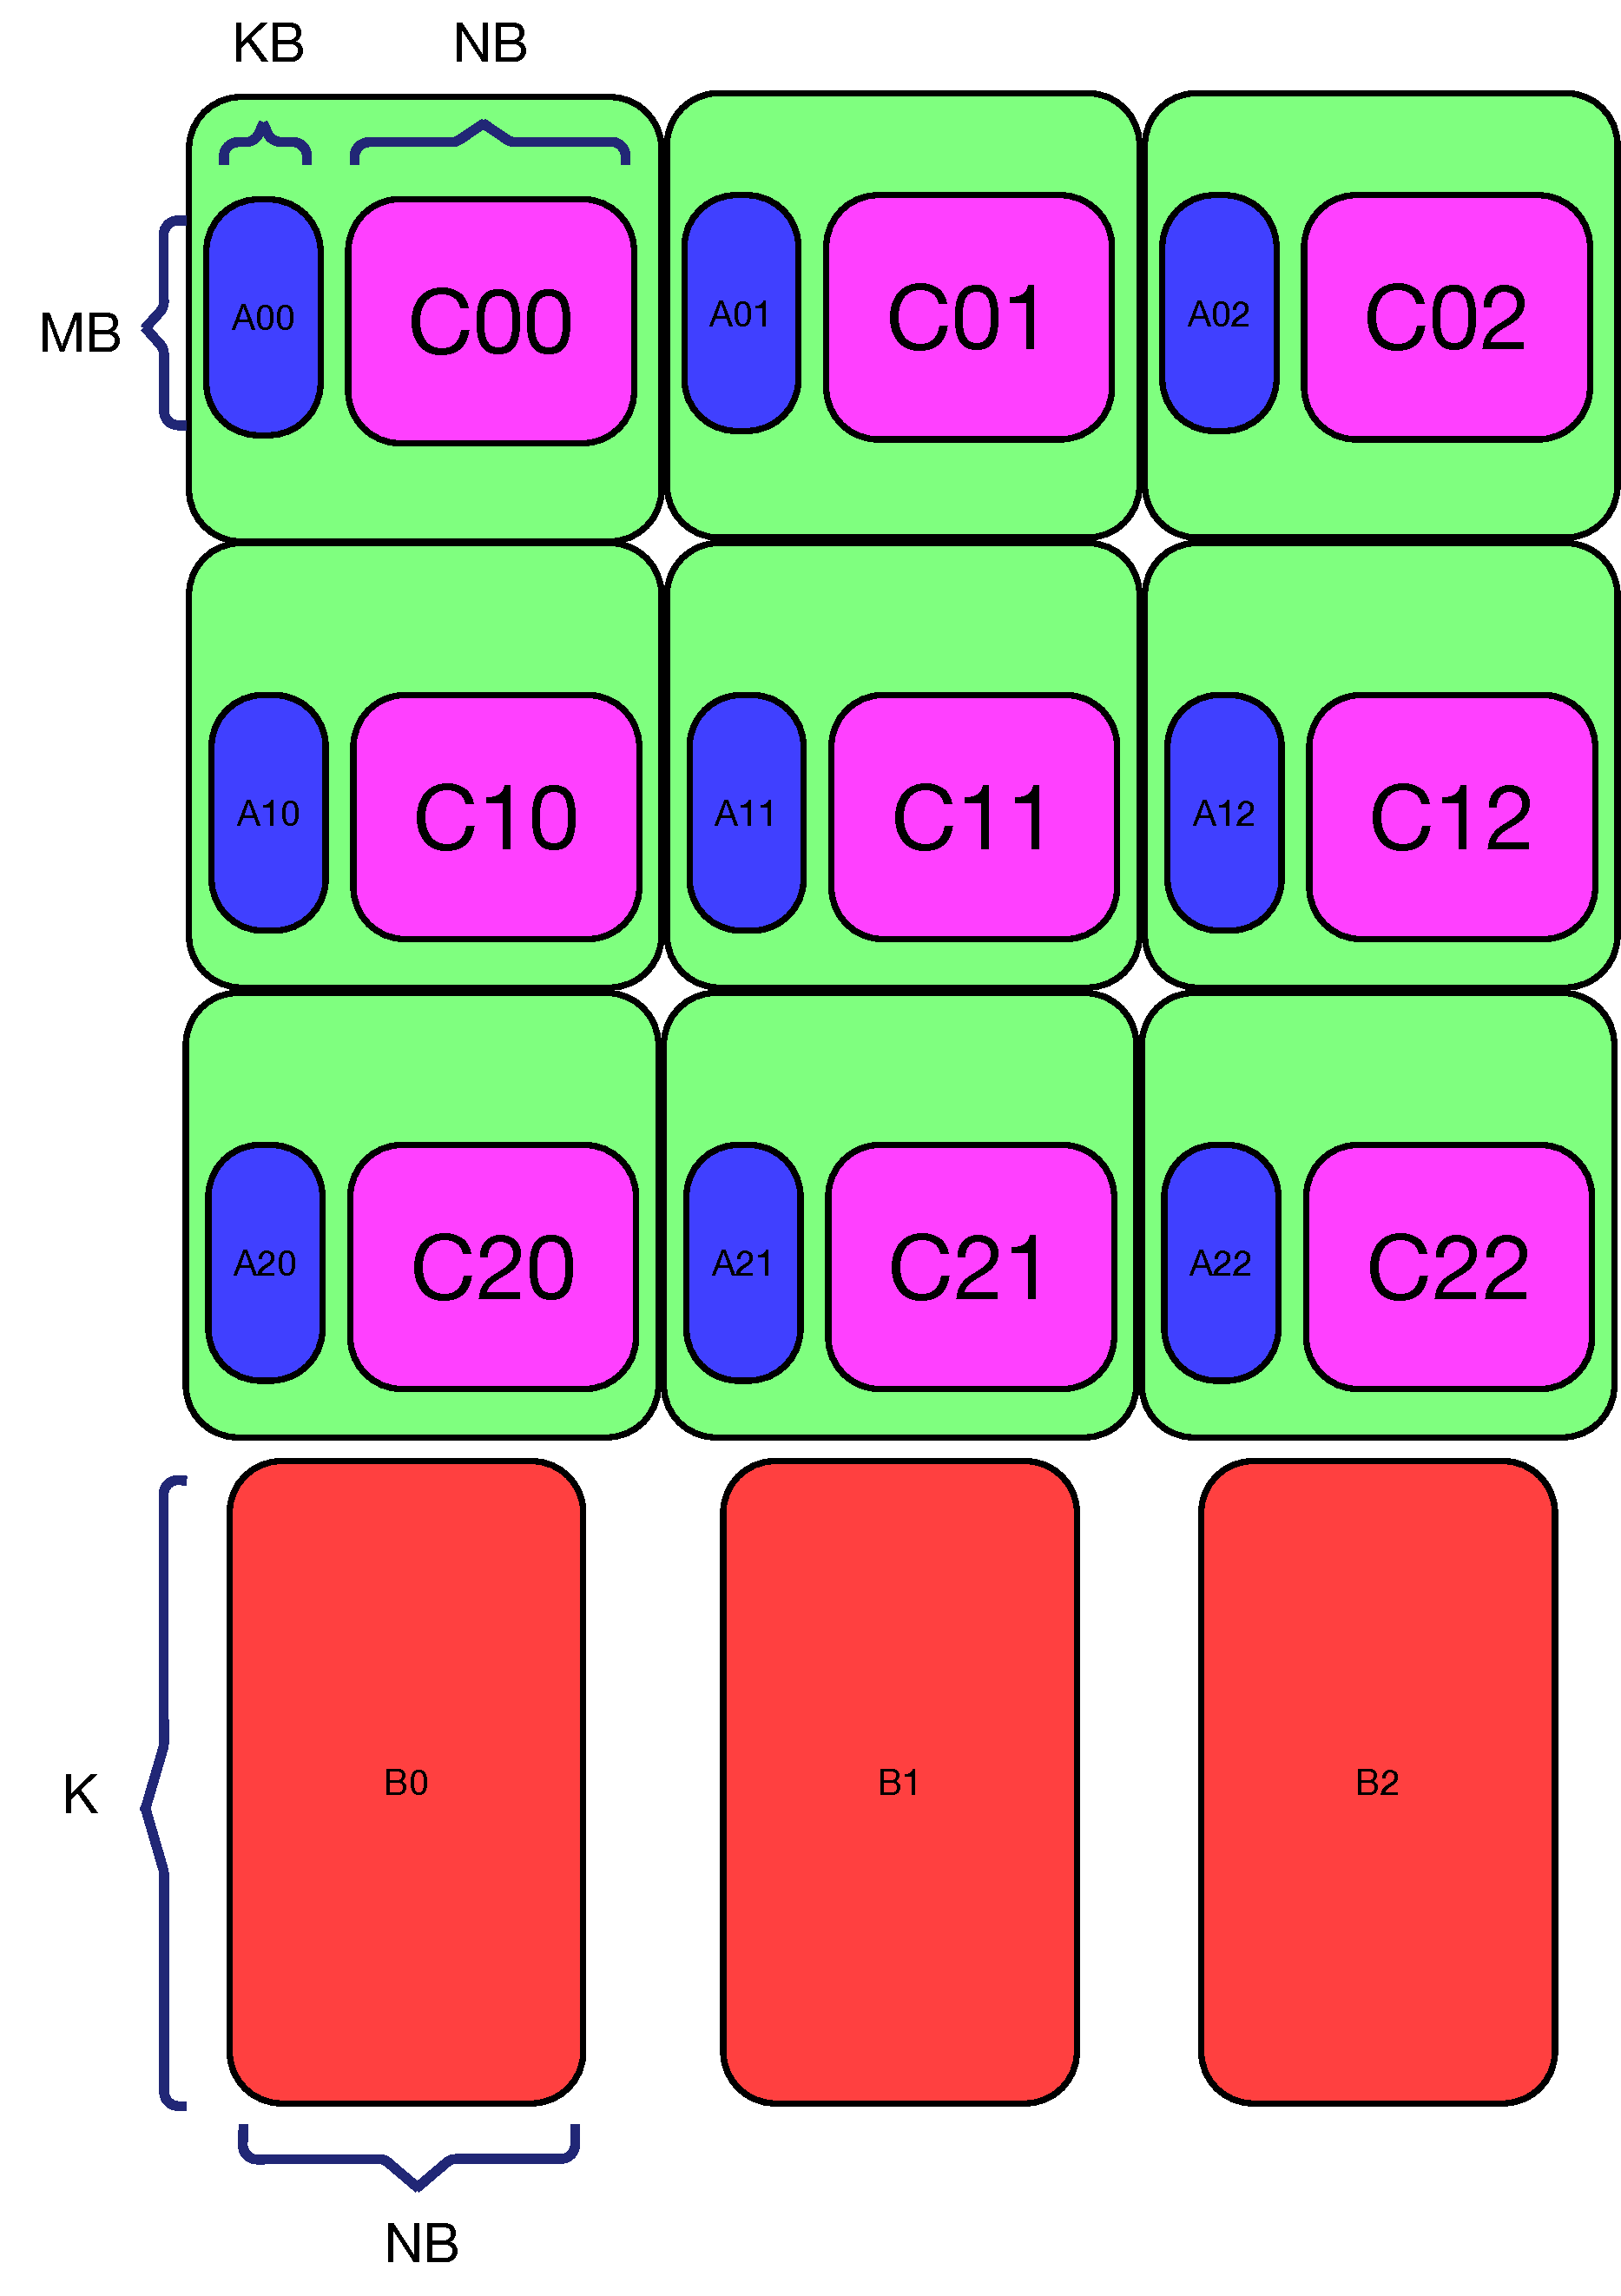
\includegraphics[width=\linewidth]{figures/gemm_A_C_memory_summa/1.pdf}
    \caption{Data distribution.}
    \label{fig:gemm_summa_1}
  \end{subfigure}
  \hfill
  %
  \begin{subfigure}{0.40\columnwidth}
    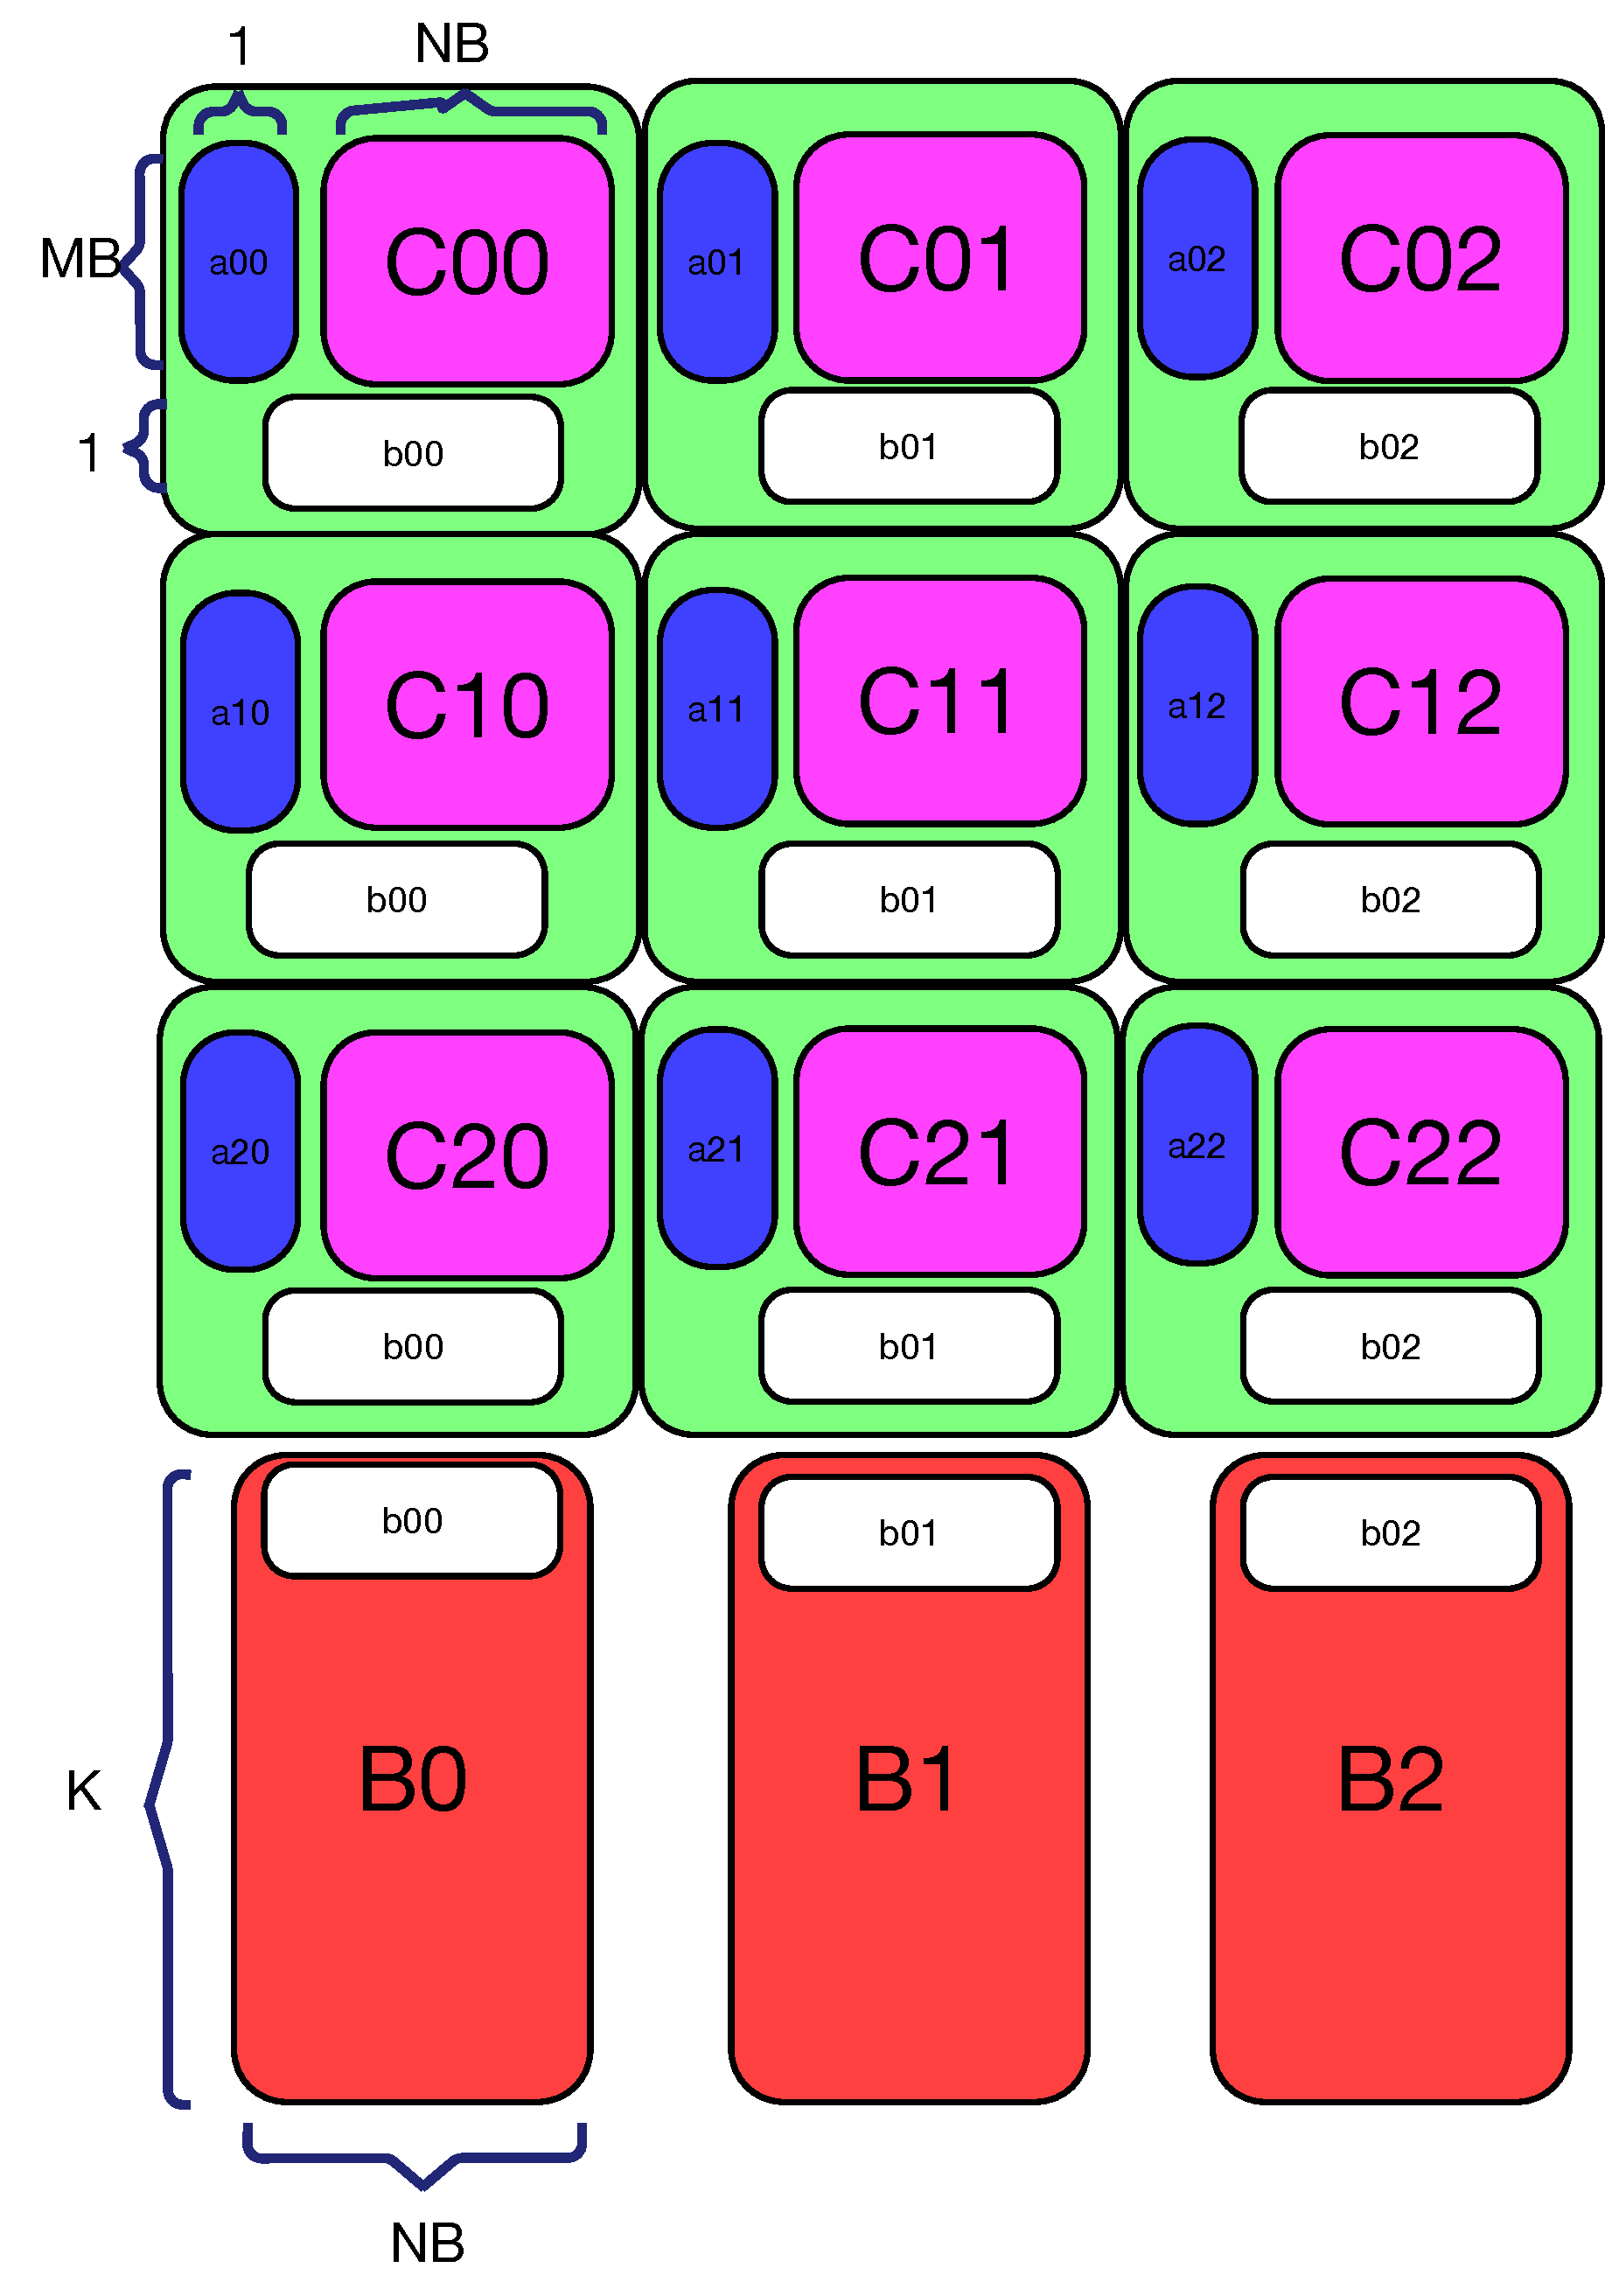
\includegraphics[width=\linewidth]{figures/gemm_A_C_memory_summa/2.pdf}
    \caption{The first iteration.}
    \label{fig:gemm_summa_2}
  \end{subfigure}
  \caption{\summa.}
  \label{fig:gemm_summa_1_2}
\end{figure}

\summa is one of the classical algorithms to solve matrix multiply problem~\cite{van1997summa}.
%
Figure~\ref{fig:gemm_summa_k0} shows the communication of the first iteration of \summa on $3 \times 3$ PEs/processes/blocks, which broadcasts $A$ horizontally, broadcasts $B$ vertically, and operates outer-produce between $A$ and $B$.
%
It can be seen that \summa consists of $K$ number of outer-product, and the vector sizes of each outer-product are $M$ and $N$.
%
Towards the special scenario where $B$ is streamed in, Figure~\ref{fig:gemm_summa_1} describes how the data is distributed, and Figure~\ref{fig:gemm_summa_2} shows the process of the first iteration, where $A$ and $C$ are distributed on $3 \times 3$ PEs ($PE_x = PE_y = 3$), $PE_x \times KB = K$, $PE_x \times NB = N$, and $PE_y \times MB = M$.


\subsection{Performance Analysis}


\begin{figure}[t!]
  \centering
  \begin{subfigure}{0.48\columnwidth}
    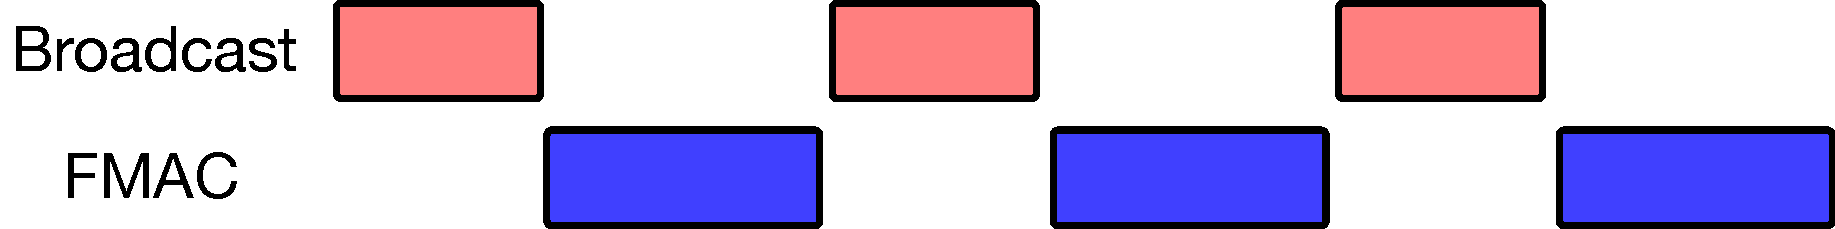
\includegraphics[width=\linewidth]{figures/gemm_A_C_memory_summa/3.pdf}
    \caption{Mathematical}
  \end{subfigure}
  \hfill
  \begin{subfigure}{0.48\columnwidth}
    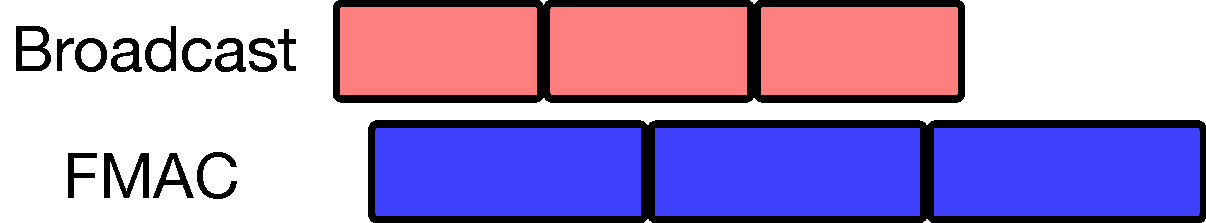
\includegraphics[width=\linewidth]{figures/gemm_A_C_memory_summa/4.pdf}
    \caption{Optimal}
  \end{subfigure}
  \caption{Execution of \summa}
  \label{fig:gemm_summa_3_4}
\end{figure}


The execution model of \summa can be described in Figure~\ref{fig:gemm_summa_3_4} regarding its mathematical definition and the optimal goal.
%
As shown above, it can be seen: (1) each outer-product is independent; (2) the tile at the top right corner is the last to execute.
%
Therefore, if considering the first iteration of that PE in FP16, the number of FMAC is $nb\_fmac = MB \times NB$, using $nb\_fmac/4$ cycles.
%
For the communication overhead, that PE needs $PE_x + MB/2$ cycles (pipelined) to receive one piece of $A$ from West and $PE_y + NB/2$ cycles (pipelined) for the weight ($B$) from South.


First, let's see the efficiency that the mathematical definition can achieve.
%
If the two broadcasts of $A$ and $B$ can not be overlapped, then, the theoretically efficiency is 
\begin{equation}
  efficiency = MB \times NB/(MB \times NB+4 \times PE_x + 2 \times MB+4 \times PE_y + 2 \times NB)
  \label{eq:summa_1}
\end{equation}
%
If that two broadcasts can be overlapped, then
\begin{equation}
  efficiency= MB \times NB/(MB \times NB+max(4 \times PE_x + 2 \times MB, 4 \times PE_y + 2 \times NB))
  \label{eq:summa_2}
\end{equation}
%
Next, let's consider the optimal one, where FMAC and the two broadcasts can be overlapped, then
\begin{equation}
  efficiency = MB \times NB/max(MB \times NB, 4 \times PE_x + 2 \times MB, 4 \times PE_y + 2 \times NB)
  \label{eq:summa_3}
\end{equation}





%\includegraphics{summa_gemm.gif}
